\documentclass[12pt, preprint]{hacked-aastex}
\usepackage{titlesec, hyperref, mdwlist, wrapfig, mdframed, enumitem}
\usepackage[style=numeric]{biblatex}

\bibliography{blanton}

\setlength{\topmargin}{0in}% 
\setlength{\headsep}{0in}% 
\setlength{\headheight}{0in}% 
\setlength{\textheight}{8.8in}% 

\newlength{\mylen}

\newenvironment{ditemize}
{ \begin{list}{}{%
\setlength{\topsep}{0pt}% 
\setlength{\partopsep}{3pt}% 
\setlength{\itemsep}{1pt}\setlength{\parsep}{1pt}% 
\setlength{\itemindent}{0pt}\setlength{\listparindent}{12pt}%
\setlength{\leftmargin}{24pt}\setlength{\rightmargin}{0in}%
\setlength{\labelsep}{3pt}\setlength{\labelwidth}{6pt}%
\setlength{\mylen}{3pt}
\renewcommand{\makelabel}{\makebox[\labelwidth][l]{\raisebox{\mylen}{\tiny$\bullet$}\hspace{\fill}}}}}
{\end{list}}


\begin{document}

\pagestyle{plain}
\titlespacing*{\section}{0pt}{0pt}{0.5\baselineskip}
\titlespacing*{\subsection}{0pt}{0.5\baselineskip}{0.5\baselineskip}
%\titleformat{\section}{\bfseries}{\thesection.}{1em}{} 

\newcommand{\imtxt}[1]{\textcolor{red}{#1}}
\newcommand{\imsout}[1]{\textcolor{red}{\sout{#1}}}

\title{{\large Characterizing the local population of mid-infrared-emitting active galactic nuclei}}

\maketitle

\renewcommand{\baselinestretch}{0.75}\normalsize
{\hypersetup{hidelinks} \tableofcontents }
\renewcommand{\baselinestretch}{1.0}\normalsize

% TODO
% - fix refs
% - How much lower luminosity?
% - Better Spitzer spectra figure

\newpage
\section{Summary}\label{sec:summary}

Unveiling the growth and development of galaxies is one of the ``prime
objectives'' of NASA's Cosmic Origins program.  Active galactic
nuclei, powered by accretion onto supermassive black holes at the
centers of galaxies, are thought to play an important role in the
evolution of galaxies by regulating and possibly quenching the
formation of stars.  For this reason, the Cosmic Origins program has a
focus on the history and evolution of supermassive black holes.  For
similar reasons, the National Academy of Sciences' Decadal Survey
report ``Pathways to Discovery in Astronomy and Astrophysics for the
2020s'' describes the study the growth of the supermassive black hole
population as essential to its priority science area, ``Unveiling the
Hidden Drivers of Galaxy Growth.''

{\bf We propose to measure the luminosity distribution of mid-infrared
  (mid-IR) emitting active galactic nuclei (AGN) and their host
  galaxies in the local universe using data from the Wide-field
  Infrared Survey Explorer, Spitzer Space Telescope, and GALEX,
  combined with ground-based data from the Sloan Digital Sky Survey IV
  (SDSS-IV; \cite{blanton17a}).}  Our work builds on the Mapping
Nearby Galaxies at APO survey (MaNGA; \cite{bundy15a}), which provides
optical integral field spectroscopy for 10,000 galaxies at redshifts
$z<0.15$.  The ultraviolet and mid-IR data available from the
aforementioned NASA projects provides a powerful window into the AGN
population and the properties of the host galaxies.

We will advance the state-of-the-art in three ways. First, we will use
a new selection criterion to {\bf increase the mid-IR AGN sample by a
  factor of three} and to extend the sample to lower Eddington
ratios. Second, we will {\bf quantify the mid-IR selection effects and
  provide upper limits for non-detections} of mid-IR AGN
luminosities. These upper limits are essential to determining the
distribution of AGN properties as a function of galaxy host property,
yet no previous analyses have calculated them or accounted for them in
analysis.  Third, using the MaNGA sample we will {\bf measure AGN host
  galaxy properties in unprecedented detail}.

This work will provide new results of fundamental importance to
understanding the nature of supermassive black hole accretion and its
effects on galaxy evolution.  Galaxy formation simulations make direct
predictions of the relationship between the AGN luminosity
distribution and galaxy properties---therefore our measurements will
have the power to distinguish between different theoretical
models. The relationship between galaxy properties, mid-IR AGN
emission, and other manifestations of AGN can also be used to
understand the fundamental structure of the central gas and dust
structure (the ``torus'') in AGN.

%\newpage
\section{Objectives \& Relevance: AGN and Galaxy Evolution}\label{sec:intro}

\fbox{\parbox{\textwidth}{\bf This proposed work will establish a new
    low redshift baseline for the distribution of AGN luminosities as
    a function of host galaxy properties that galaxy formation
    theorists can use as a new observational constraint. In this
    section we explain the theoretical context that makes this work
    significant and important.}}

A central question in galaxy formation is why the most massive
galaxies have not converted more of their available baryons into
stars, and instead have ended their star formation. This question has
existed since the 1970s \cite{white78a}.  In modern $N$-body and
hydrodynamic simulations the details are different but the problem is
the same: the halo mass function extends nearly as a power law to high
masses, but the galaxy stellar mass function cuts off exponentially.
Without a way to prevent star formation in the highest mass halos
these two functions should follow each other more closely
\cite{benson03a, somerville15a}.

Among the many possible solutions, the most favored is AGN that in
massive galaxies somehow prevent their continued growth
\cite{fabian12}. AGN efficiently generate radiation, jets, and winds,
the effects of which are indeed observed and can provide negative
feedback to star formation.  The $M_{\rm BH}$--$\sigma$ relation
appears to point to some sort of co-evolution of galaxies and their
black holes \cite{kormendy04b}. Only with AGN feedback can simulations
reproduce the quenched massive galaxy fraction and the stellar mass
function \cite{somerville15a, wellons22a}.

This situation, however, is not ``case closed.'' The hydrodynamic
simulations each have their AGN feedback and other parameters tuned to
fit observations like quenched fractions and stellar mass functions,
and each have sometimes dramatically different methods for applying
AGN feedback. So we need distinct observations to test which, if any,
of these theories of AGN feedback describes the real universe. An
important prediction is the distribution AGN luminosities as a
function of host galaxy properties \cite{habouzit22a}.

\begin{table}[b!]
\caption{\label{table:feedback} 
The Variety of AGN Feedback Methods In Cosmological Simulations\\ ~}
\begin{tabular}{|c|c|c|c|}
\hline
Simulation & Eddington Ratio Criterion & High $\lambda$ Mode & Low $\lambda$ Mode \cr
\hline
\hline
Illustris \cite{sijacki15a} & 0.05 & Thermal & Thermal \cr
IllustrisTNG \cite{weinberger17a} & 0.002---0.1 & Thermal & Kinetic \cr
Horizon-AGN \cite{dubois14a} & 0.01 & Thermal & Kinetic \cr
SIMBA \cite{dave19a} & 0.2 & Kinetic & Kinetic \cr
EAGLE \cite{schaye15a} & --- & \multicolumn{2}{c|}{Thermal} \cr
NIHAO \cite{blank19a} & --- & \multicolumn{2}{c|}{Thermal} \cr
\hline
\end{tabular}
\end{table}

The simulations do not follow black hole seeding, growth, and AGN
feedback from first principles; they require subgrid prescriptions.
Black hole accretion is modeled with Bondi-Hoyle-Lyttleton accretion
\cite{edgar04a}, with details varying between simulations.  These
models determine the Eddington ratio $\lambda$ between the accretion
rate and the Eddington rate, the maximum rate for spherical accretion.
Two basic types of AGN feedback are implemented: thermal feedback and
kinetic feedback, which can depend on $\lambda$. Table
\ref{table:feedback} summarizes how these are used by different
simulations, which illustrates the variety of assumptions made.  As an
example, IllustrisTNG uses thermal feedback at high $\lambda$,
corresponding to the observational radiative/thermal/quasar mode, and
uses kinetic feedback for at low $\lambda$, corresponding to the
observational kinetic/jet/radio mode.

Although these simulation recover basic scaling relations of galaxies
well, their predictions vary dramatically in Eddington ratio
distributions and their dependence on on stellar mass
\cite{habouzit22a}. Some of the Eddington ratio distributions shift
higher with mass, some decrease, some are non-monotonic.  These
differences can provide a critical test of galaxy formation models.

The work of \cite{habouzit22a} underscores difficulties in comparing
this prediction to observations. AGN feedback models need to be
converted into observables, which typically are X-ray luminosity,
broad line emission, narrow line emission, IR emission, and radio
emission. X-ray and optical line emission is further modified by dust
obscuration in the surroundings of the AGN. These difficulties
motivate the better observational understanding the joint distribution
of these multiwavelength signatures of AGN.

But the statistical distribution of AGN luminosities as a function of
galaxy properties is poorly understood, because the selection effects
on the existing samples have not been well characterized. In this work
we concentrate on one aspect of this problem, characterizing the
distribution of mid-IR-detected AGN, which are less susceptible to
obscuration.  We propose to unveil a larger population of mid-IR
emitting AGN than it was previously possible to reliably detect, and
to also set accurate upper limits on mid-IR AGN emission for galaxies
without detected AGN. From these measurements we can determine the
luminosity and Eddington ratio distributions of AGN as a function of
galaxy properties.  These observations will establish an important new
low redshift constraint on galaxy formation simulations.

\section{Scientific Impacts: AGN host galaxies and Eddington ratio distributions}\label{sec:intro}

\fbox{\parbox{\textwidth}{\bf This work will establish more firmly
    than previously possible the relationship between mid-IR AGN and
    their host galaxies in the local universe. In this section, we
    explain how the measurements we propose will advance the state of
    the art.}}

The major goal which this work contributes to is to constrain the
distribution of AGN luminosities as probed in many ways (e.g. radio,
mid-IR, optical narrow lines, and X-rays) as a function of stellar
mass $M_\ast$, velocity dispersion $\sigma_v$, and star formation rate
(SFR):
\begin{equation}
\label{eq:model}
\Phi\left(L_{\rm radio}, L_{\rm IR}, L_{\rm OIII}, L_X | M_\ast, \sigma_v, {\rm SFR}\right),
\end{equation}
Surprisingly, observational constraints on this distribution are not
as well-understood as they could be, and much of the literature on the
subject is riddled with difficult-to-understand selection effects
(e.g. \cite{trump15a, jones17a, hviding22a}).

The problem is that AGN manifest in a variety of different ways,
depending both on their intrinsic state and on the viewing angle of
the observer, and across all wavelengths of light.  To make things
more complicated, their signatures are often in competition with
stellar emission and interstellar gas emission.  But the understanding
of the AGN distribution is further hampered by the way that it is
typically studied. Most AGN demographic focus on identifying AGN
(\cite{kauffmann03b, lacy15a, sanchez19a, comerford20a, greene20a})
but {\it do not} determine the upper limits on luminosity caused by
effects of host galaxy contamination (\cite{trump15a, jones17a} being
rare exceptions). This approach clearly throws out important
information, and also makes the resulting analyses susceptible to
untracked selection effects. It makes it impossible to study the
population of low luminosity AGN accurately, since whether a given low
luminosity AGN is identifiable largely depends on the host galaxy
properties.

Here we propose to advance the understanding of the distribution of
mid-IR AGN luminosities $L_{\rm IR}$ and Eddington ratios, and its
dependence on host galaxy properties, at low redshifts.  We will
measure the mid-IR AGN-related luminosities for detected AGN {\it and}
upper limits for galaxies without detected AGN. We will create a new,
larger sample and probe lower luminosity and Eddington ratio AGN than
were previously identified in low redshift samples.

{\bf New and archival observations of the low redshift universe
  present an opportunity to make progress on these
  questions}. Specific motivations for revisiting this question are:
\begin{ditemize}
\item With the Sloan Digital Sky Survey's Mapping Nearby Galaxies at
  APO (MaNGA) program, we can measure low redshift galaxies
  exquisitely well, and separate spatially the AGN and galaxy emission
  (\cite{bundy15a, blanton17a}).  Our analysis takes advantage of
  10,000 potential AGN host galaxies from MaNGA with high
  signal-to-noise ratio measurements of stellar mass, velocity
  dispersion, SFR, and other parameters.
\item Existing surveys in the mid-IR from the Wide-field Infrared
  Survey Explorer (WISE; \cite{wright10a}) are well matched to find
  mid-IR AGN in MaNGA galaxies \cite{comerford20a}. But previous
  searches for AGN in WISE have focused on the most extreme AGN,
  whereas lower Eddington ratio AGN are readily identifiable but have
  not been studied previously.
\item The Spitzer Space Telescope archive has mid-IR spectroscopy of
  galaxies in MaNGA and other nearby galaxies, which we can use to
  validate the lower Eddington ratio cases and to study more detailed
  properties of the mid-IR emission.
\end{ditemize}

The well-measured MaNGA host galaxies present a unique opportunity
relative to other AGN samples. The mid-IR-based bolometric luminosity
distribution of AGN and its evolution has been measured with massive
samples of AGN selected in the mid-IR \cite{lacy15a}. However, it is
ambiguous how these AGN relate to their underlying host galaxies and
the black holes themselves, because relatively little can be inferred
about the host galaxies, which are faint, poorly resolved, and often
outshone by the AGN.  This difficulty also makes it hard to to account
for mass-dependent effects, such as lower metallicity with PAH
emission and hotter dust masquerading as AGN \cite{hainline16a,
  sajina22a}.

In this work, we will utilize these new resources to answer the
critical question of how AGN populate host galaxies in the low
redshift universe. {\bf The direct impact of this work will be to}:

\fbox{
\begin{minipage}{0.9\textwidth}
\begin{ditemize}
    \item Expand the potential sample of mid-IR emitting AGN in the
      local universe by a factor of three, and extending to lower
      Eddington ratios and luminosities, by validating a new selection
      technique.
    \item Measure the luminosity and Eddington ratio distribution of
      mid-IR emitting AGN as a function of stellar mass, velocity
      dispersion, and star formation rate, as an observational
      constraint on galaxy formation theory.
    %\item Explore the relationship between mid-IR and optical narrow
    %  line manifestations of AGN.
\end{ditemize}
\end{minipage}
}

This work will have long term indirect impacts as well. The selection
technique we develop will be applicable for use in larger samples
(with less information per galaxy) such as the SDSS Legacy Survey and
the DESI Bright Galaxy Survey. Doing so would massively increase the
power of the legacy WISE data set for the purposes of selecting AGN in
the local and more distant universe.

\section{Methods of Proposed Work\label{sec:methods}}

To advance our understanding of AGN in the local universe, we use the
following methods:
\begin{ditemize}
    \item We use a low redshift sample of galaxies from MaNGA with 
    jointly analyzed WISE data (the MaNGA NASA Sloan Atlas or MNSA)
    (Section \ref{sec:mnsa}).
    \item We use a newly developed, more sensitive criterion to 
    identify mid-IR AGN (Section \ref{sec:criterion}).
    \item We use SED modeling methods to derive the mid-IR AGN
      luminosities and upper limits for all 10,000 MaNGA galaxies
      (Section \ref{sec:measurements}).
    \item We analyze Spitzer Space Telescope spectra to validate our 
    classifications and measurements of mid-IR (Section
    \ref{sec:spitzer}).
    \item We perform a maximum likelihood analysis using mid-IR AGN luminosities 
     and upper limits to constrain the Eddington ratio  distribution as a 
     function of galaxy properties (Section \ref{sec:erd}).
    %\item We compare the mid-IR AGN luminosity distribution to other manifestations 
    %of AGN in this sample (Section \ref{sec:other}).
\end{ditemize}

\subsection{The MaNGA NASA Sloan Atlas}
\label{sec:mnsa}

MaNGA comprises the best understood sample of 10,000 galaxies in the
universe, with comprehensive integral field spectroscopy in the
optical, constraining galaxies' central velocity dispersion, star
formation history, ionized gas properties, and dynamics. WISE
photometry detects every MaNGA galaxy and provides important
information about their AGN and star formation activity that we will
make use of here. {\bf We will make use here of a previously created
  joint photometric analysis of GALEX, DESI Legacy Imaging Surveys,
  MaNGA, and WISE data obtained in private communication, which we
  call here the MaNGA NASA Sloan Atlas (MNSA)}.

MaNGA provides an immense amount of ancillary information,
unparalleled in any other sample of its size. We need not perform any
MaNGA analysis under this grant, but can rely on already-published
analyses. MaNGA spectroscopy extends out to at least 1.5$R_e$ for
every observed galaxy, allowing inference of reliable stellar masses
and star formation rates from stellar population analysis
\cite{sanchez22a}, dynamics (e.g. \cite{graham18a}), ionized gas
properties (e.g., \cite{belfiore17a}), and many other properties.
These galaxies have a median redshift of $z\sim0.03$, with the sample
extending out to $z\sim 0.15$, and the physical spatial resolution is
typically around 1--2 kpc. They have been selected in a well-defined
way as a function of mass and color, so that each MaNGA Main Sample
galaxy's relative probability of having been observed is known, making
the sample suitable for statistical study \cite{wake17a}.

This sample has important advantages for conducting a statistical
study of AGN with low redshift galaxies.  Star formation rates over
the past 100 Myrs can be inferred from the stellar population
analysis, avoiding dependence on UV or H$\alpha$ emission, which can
be contaminated by the presence of an AGN. The high signal-to-noise
ratio stellar velocity dispersion maps provide an estimate of the
central black hole using the $M_{\rm BH}$-$\sigma$ relationship
\cite{kormendy04b}. The narrow line measurements allow us to find
nuclear narrow line regions as well as extended narrow line regions
and outflows. The sample is low enough redshift that essentially every
galaxy has informative detections in all WISE bands.

As argued by \cite{aird12a} in the context of X-ray selection, by
starting with a well-understood galaxy sample we avoid the biases
associated with samples {\it selected} to be AGN, for which the host
galaxy properties are biased at best but often inaccessible
entirely. Only by starting with a galaxy sample can we constrain the
dependence of AGN properties on galaxy properties in an unbiased way.

\subsection{Identifying AGN in WISE: A New Criterion}
\label{sec:criterion}

{\bf We propose to test and use a more inclusive AGN selection
  criterion using WISE photometry and MaNGA star formation rates that
  promises to provide around a factor of three more AGN than the
  previous standard criteria.}

AGN often exhibit mid-IR emission from dust in the periphery of the
accretion disk heated to close to sublimation temperatures,
considerably hotter than dust temperatures in star forming regions.
The W1$-$W2 color (i.e. the 4.6 $\mu$m to 3.4 $\mu$m flux ratio) is
sensitive to this AGN emission because stellar populations have a
roughly uniform W1$-$W2 color (those bands are in the Rayleigh-Jeans
regime).  Meanwhile, dust heated by star formation does not get to
high enough temperature to contribute much to W2, nor do most PAH
lines.  The W1$-$W2 color of a host galaxy is closely related to its
star formation rate (or from its W2$-$W3 color \cite{hviding22a}).
Therefore, a W1$-$W2 color redder than the expectation given the star
formation rate indicates the presence of hot dust from an AGN.

Figure \ref{fig:wise} illustrates these effects, showing the
relationship between this color and the specific SFR (sSFR) of MaNGA
galaxies from \cite{sanchez22a}.  At low W1$-$W2, there is a tight
sequence of points with a clear sSFR dependence; for these galaxies,
both bands are dominated by the host galaxy.  For the reasons
described above, the presence of an AGN and its attendant hot dust
leads to redder W1$-$W2, and the ``spray'' of points above the tight
sequence are likely to be AGN.

\begin{figure}[t!]
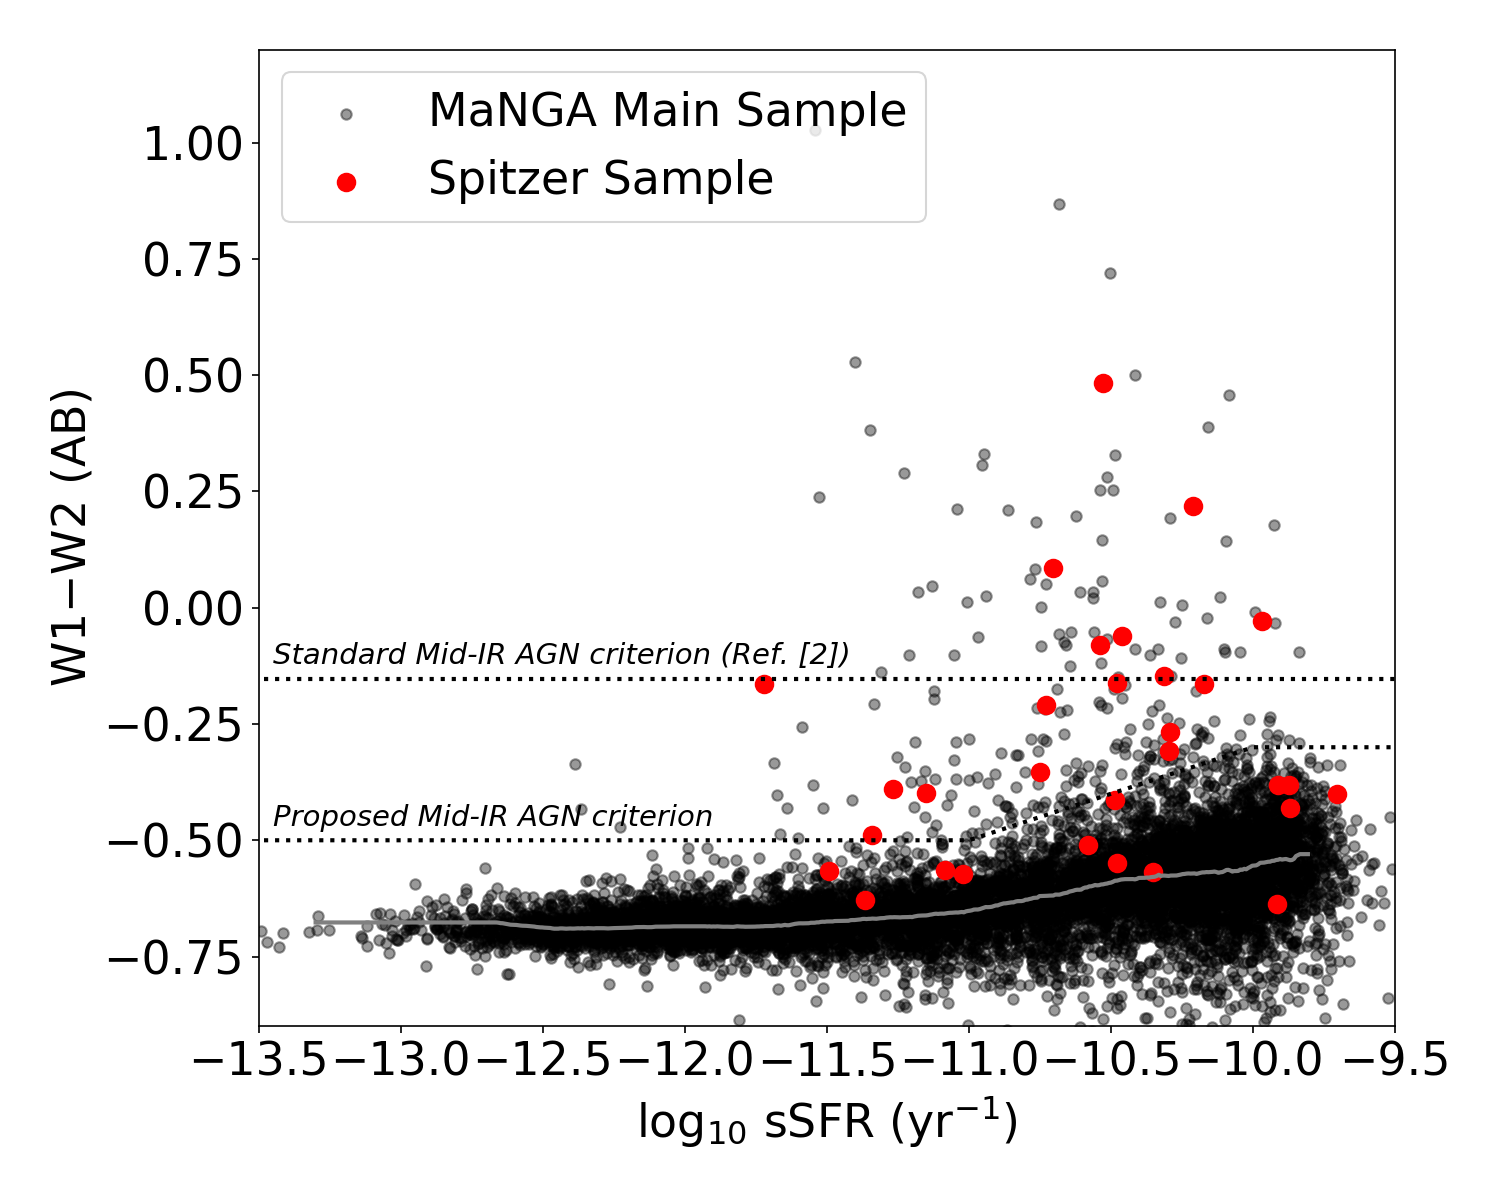
\includegraphics[width=0.64\textwidth]{w1w2-vs-ssfr.png}
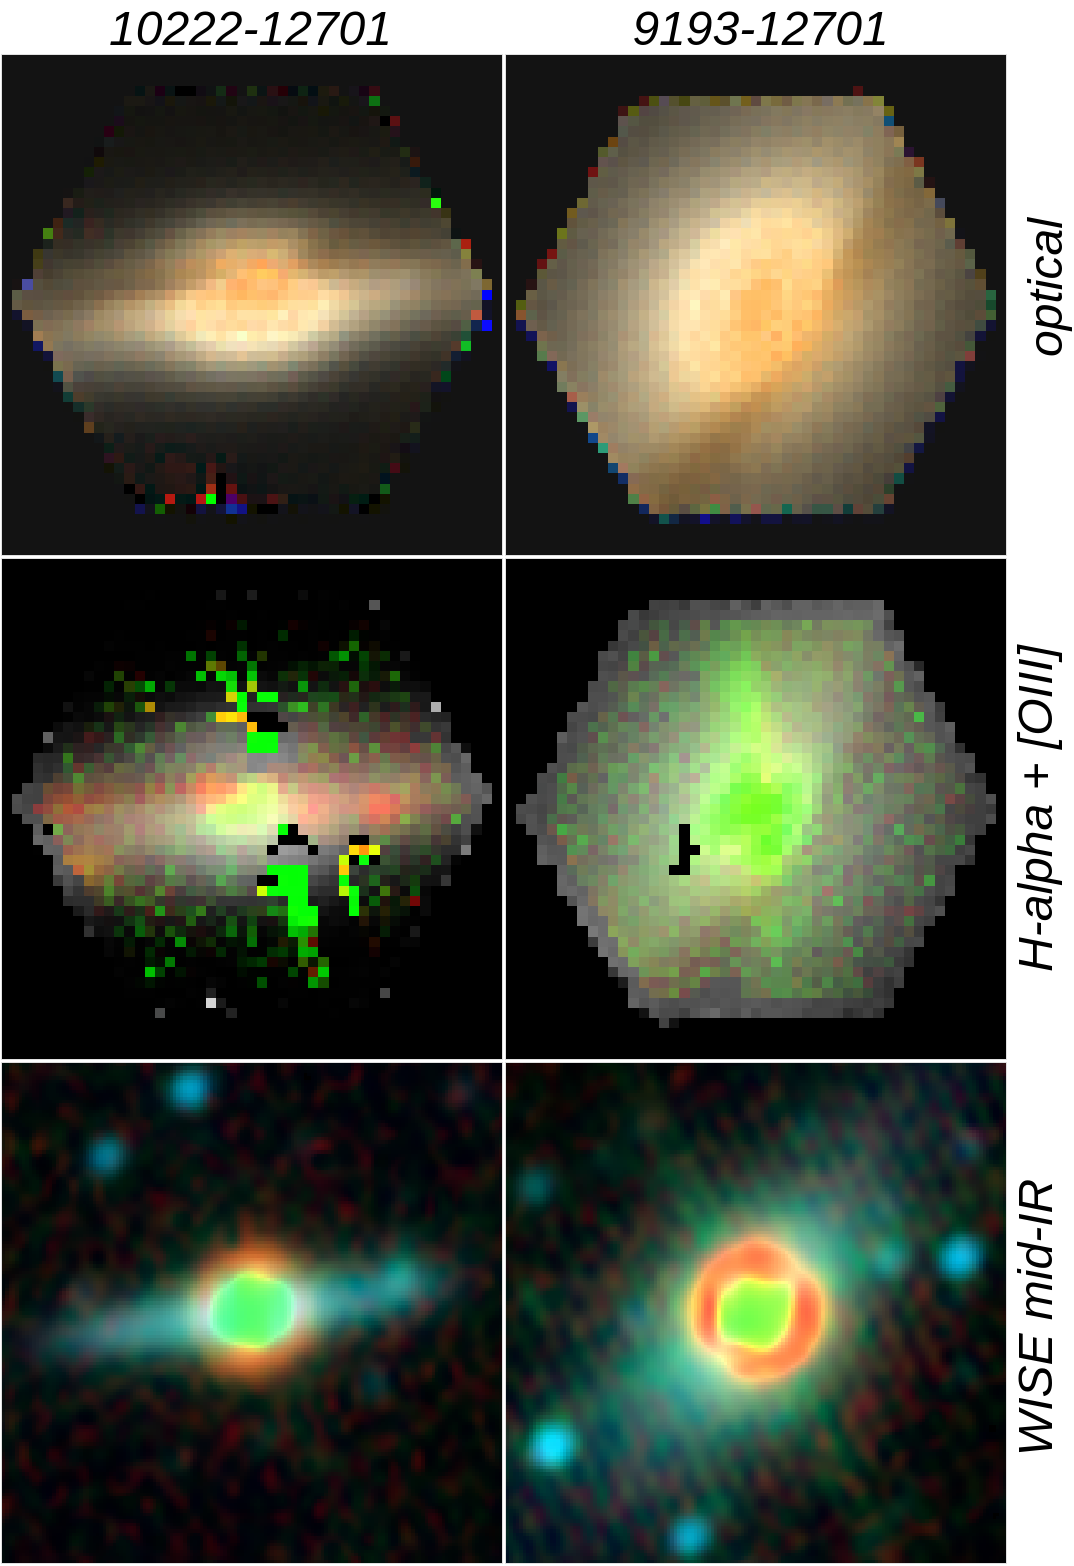
\includegraphics[width=0.35\textwidth]{ir-grid.drawio.png}
  \vspace{-22pt}
    \caption{
\label{fig:wise} \small Mid-IR AGN detection. 
The left panel shows W1$-$W2 colors (AB) of MaNGA galaxies vs star
formation rate determined from the optical stellar population fits.
The dotted line is the commonly used AGN criteria from
\cite{assef18a}. The grey line is designed to follow the dependence of
W1$-$W2 on SFR, and (with care taken to validate it) will provide a
more complete census of mid-IR AGN from MaNGA. The right panel shows
two example AGN selected in the mid-IR, with one that only passes the
proposed new criterion and one that passes both criteria. The top
shows the optical broadband color image; the middle shows the optical
broadband light as grey, with [OIII] emission overlaid as green and
H$\alpha$ emission overlaid as red; the bottom shows the WISE mid-IR
color image. The newly included galaxy is an AGN based on its [OIII]
emission and morphology.}
\end{figure}

The upper dotted line shows the typical criterion used to select AGN
(specifically, the most inclusive criterion from from \cite{assef18a},
here translated to AB magnitudes). However, there are many objects in
between this criterion and the sequence of non-AGN. The reason that
\cite{assef18a} and almost all other references choose such
conservative criteria even in their most inclusive samples is that
typically they do not know much about the host galaxy properties.  The
vast majority of WISE-detected AGN do not have a redshift and
therefore no appropriate $K$-correction. The observed-frame W1$-$W2
colors, without any known host galaxy color to compare to, is much
less informative and therefore the criterion used must be much more
conservative. Except in the case of \cite{hviding22a}, all alternative
criteria to those in \cite{assef18a} are more conservative and include
even fewer candidates \cite{jarrett11a,stern12a}.

For the MaNGA-based sample, we do not have these difficulties and can
define a criterion that hews more tightly to the intrinsic host galaxy
distribution, shown as the lower dotted line. This new criterion
increases the mid-IR emitting AGN candidate sample by a factor of
three.

We will further refine this selection using other MaNGA-based
measurements such as stellar metallicity, stellar mass, velocity
dispersion, or Balmer decrement, and the W2$-$W3 color
\cite{hviding22a}, to help predict the host galaxy W1$-$W2
distribution.  

\subsection{Measuring mid-IR AGN luminosities and upper limits}
\label{sec:measurements}

{\bf For every galaxy in MaNGA we will use SED modeling techniques to
  determine either: (a) measured mid-IR AGN luminosities at 6 $\mu$m
  and 15 $\mu$m, if an AGN is identified, or (b) an upper limit on the
  mid-IR AGN luminosity, if an AGN is not identified.  These upper
  limits have never previously been determined.}

A considerable fraction---more than half in some cases---of the W2
luminosity measured by WISE for any AGN is from the host galaxy
itself.  This holds even for the extreme mid-IR AGN selected by
\cite{assef18a}; their W1$-$W2 values are only 0.5--2 mag redder than
the host galaxy sequence.  It is essential to account for the
contamination due to the host galaxy. For this reason many previous
studies such as \cite{hviding22a} have not calculated mid-IR-based
luminosities for objects like those in our sample.

% We can crudely estimate the mid-IR AGN luminosity in W2 by using the
% excess W1$-$W2 over the grey line in Figure \ref{fig:wise}.  If we
% assume the entire excess is due to the AGN contribution to W2, and
% that it makes no contribution to W1, we can infer the AGN
% contribution to W2. We then can convert that W2 flux to a 6 $\mu$m
% luminosity using the AGN SED from \cite{richards06a} or from one of
% the typical AGN SEDs that we fit below from \cite{nenkova08a}.
% Similarly, we can calculate a crude estimate of an upper limit on
% the AGN luminosity by using the difference between the grey line and
% our color criterion for the sSFR of any particular galaxy; this will
% tell us how much AGN luminosity would be necessary to classify that
% galaxy as an AGN.  These crude estimates have the virtues of
% simplicity and model independence.

We do so here using SED fits including both AGN and star formation
components. We will use a non-negative fit to a large set of simple
stellar population (SSP) templates from the Flexible Stellar
Population Synthesis models (FSPS; \cite{conroy09a}), along with a
broad set of AGN templates from the ``Clumpy'' models
\cite{nenkova08a}. The SSPs span a grid of ages, metallicities, and
dust attenuation and emission properties. The Clumpy models span a
range of values for $\tau_V$, the number of clouds, and the
distribution of clouds. Performed with a Python version of the {\tt
  kcorrect} software \cite{blanton07b}, these nonnegative fits are
extremely fast, taking a fraction of a second per galaxy.

Examples of some of these fits from our preliminary analysis of the
MNSA sample can be seen in Figure \ref{fig:fits}. This figure
illustrates two points: (a) that the AGN hot dust emission reddens the
W1$-$W2 color, and (b) that the AGN can be clearly detectable while
still being a minority contributor to the W2 flux.

We will characterize the luminosity of the AGN component at several
wavelengths, concentrating primarily on 6 $\mu$m and 15 $\mu$m,
commonly used reference points. We will use our error analysis (see
below) to determine which wavelengths are most strongly constrained in
the presence of modeling uncertainty and thus most suitable for
bolometric luminosity estimates.

For the MaNGA sample of bright galaxies, we anticipate that the 15
$\mu$m luminosity will be much better measured and less contaminated
by the host galaxy.  But for larger, deeper samples that are based on
matching WISE to SDSS or DESI's Bright Galaxy Survey \cite{assef18a,
  hviding22a}, we anticipate that W3 and W4 will not be well enough
measured for good constraints on 15 $\mu$m.  With this in mind, we
will determine the relationship between the 6 $\mu$m and 15 $\mu$m AGN
luminosities within MaNGA, so that that relationship can be used to
bootstrap 6 $\mu$m measurements made with larger samples.

\begin{figure}[t!]
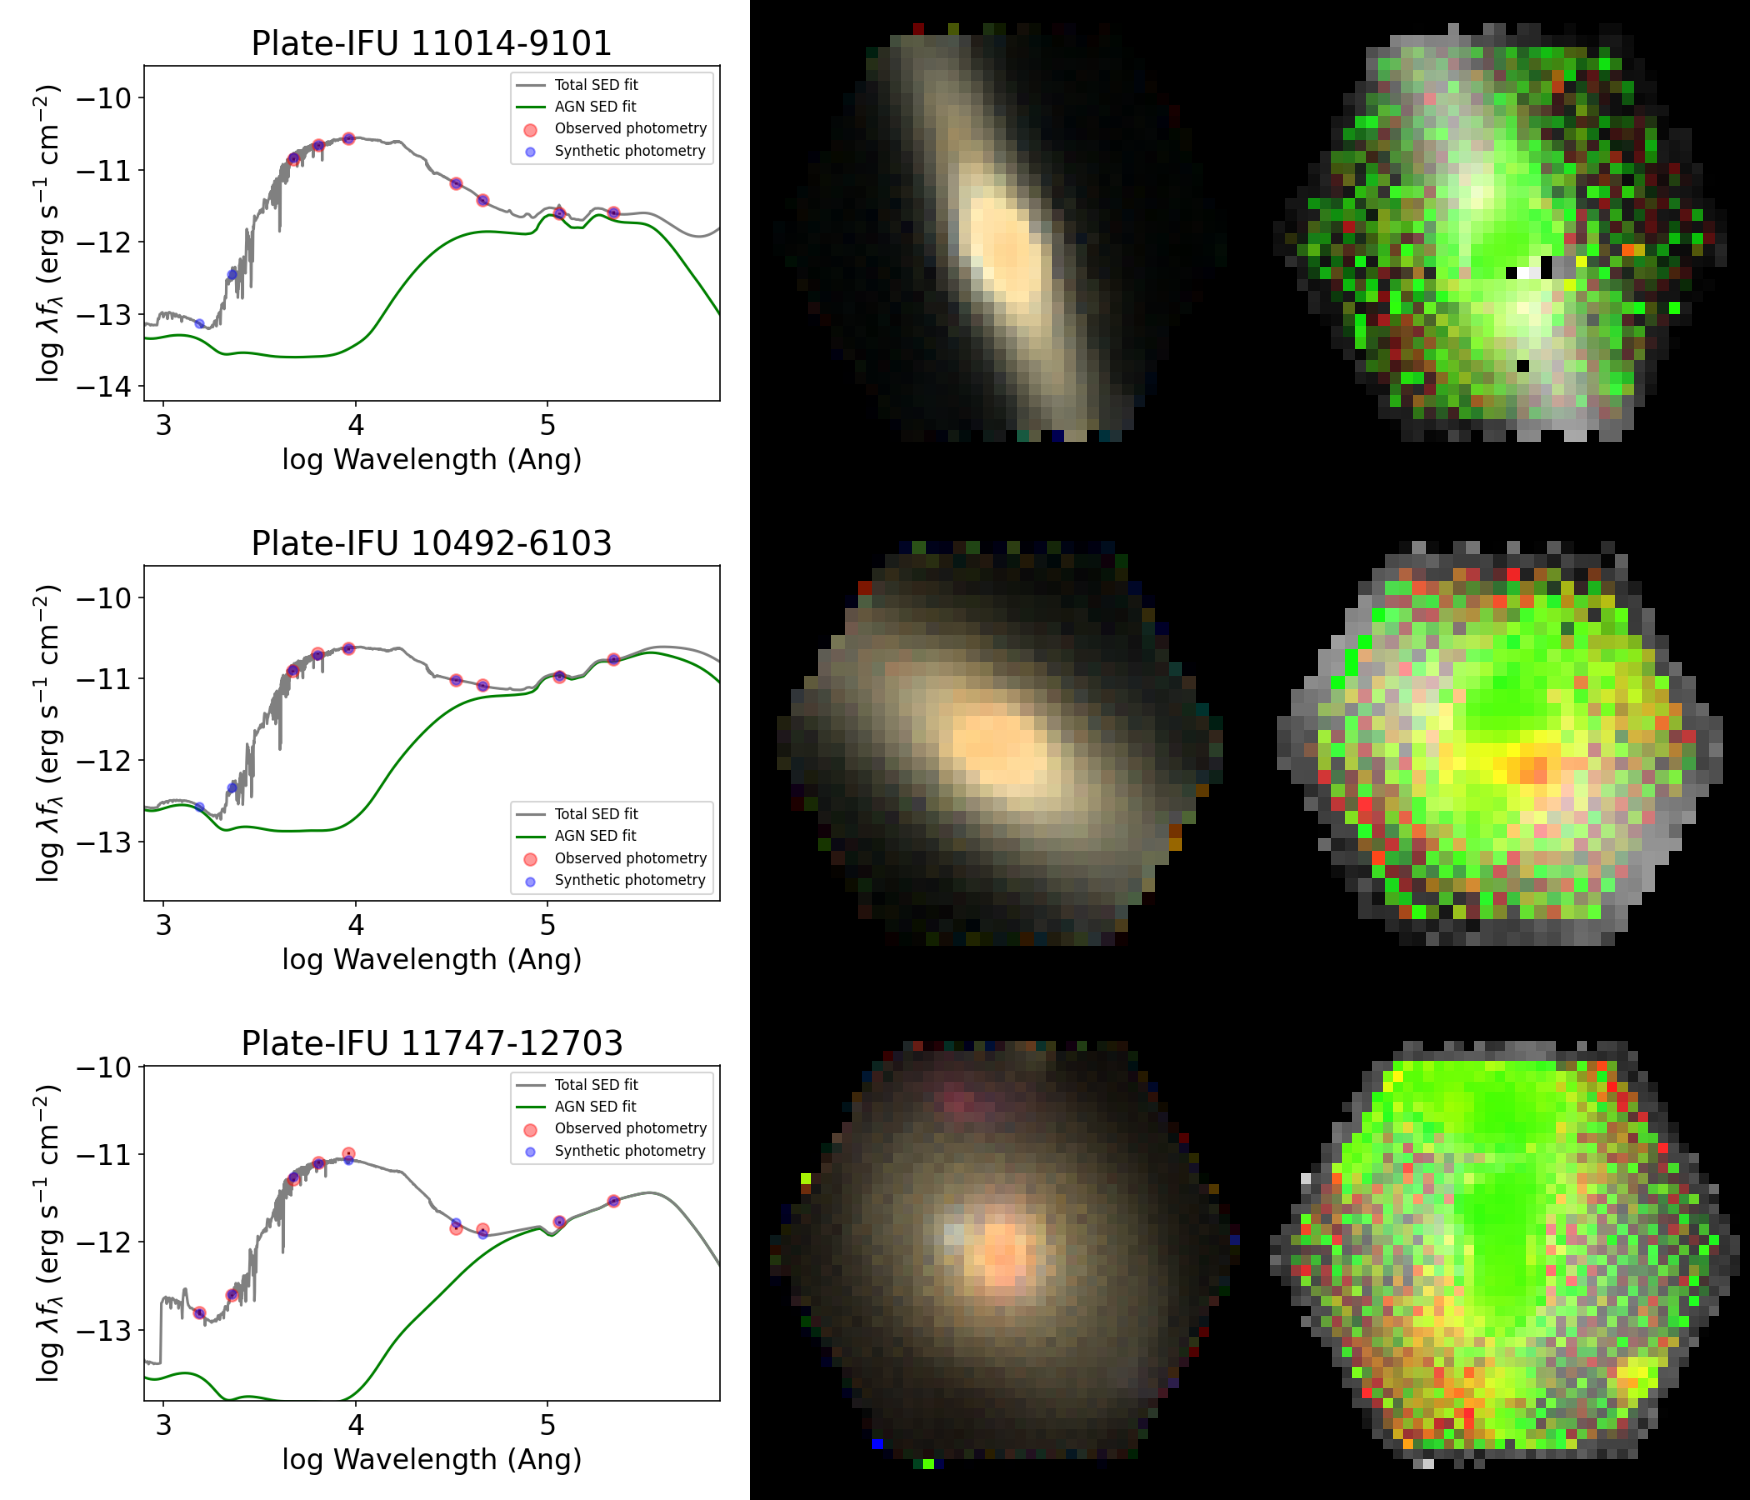
\includegraphics[width=0.98\textwidth]{spec-grid.png}
    \caption{
\label{fig:fits} \small SED fits to identified AGN. Each row
corresponds to a mid-IR detected AGN. On the left is shown the
broad-band photometry along with our preliminary SED fits.  The grey
line shows the total SED including the stellar populations, emission
lines, dust emission from the ISM, and AGN emission. The green line
just shows the contribution from AGN. The models show that AGN
contribution in the mid-IR needs to account for the stellar
contributions. On the right are the broad-band color and emission line
images from MaNGA as described in Figure \ref{fig:wise}.}
\end{figure}

For galaxies with identified AGN, our use of our fast SED fitting
technique makes it straightforward to calculate uncertainties and
upper limits. We will perform a large set of Monte Carlos on the data
set, adding random errors to the fluxes of each galaxy based on the
measurement uncertainties. The resulting distribution of Monte Carlo
AGN luminosities provides an estimate of the errors that accounts for
the statistical errors and for the wide variation we allow in the AGN
and stellar population models.

For galaxies without identified AGN, we can use the best fit SED to
help determine the upper limit. First, we will determine a ``typical''
AGN SED from the fits to galaxies with mid-IR AGN; we will also
determine this typical AGN SED as a function of each of sSFR, stellar
mass, and Eddington ratio to test for systematic variations with any
of those properties. Second, for each galaxy with no identified AGN we
can determine how much typical AGN SED can be added to its best fit
SED before it crosses our color threshold for AGN. The total mid-IR
AGN luminosity in the model that just crosses the threshold is our
estimate of the upper limit.

There are inherent uncertainties in the SED fitting process related to
our understanding of the SED models. We will explore the effects of
varying the AGN and stellar population SED grids on our results to
test their robustness.  As described in the next section, we will
further test this fitting procedure with the detailed spectra from
Spitzer. This testing procedure may lead to adjustments in the
underlying grid of SED models we use for our final results.

%Eddington ratio about 0.6 dex lower than the standard AGN as selected
%by \cite{assef18a}.

\subsection{Analysis of Spitzer Space Telescope Spectra}
\label{sec:spitzer}

{\bf To assess the accuracy of our broad band WISE data analysis, we
  will analyze the AGN signatures and spectral shape found in Spitzer
  Space Telescope spectra in the mid-IR compiled by \cite{lambrides}.}
Of their full sample, 560 spectra are of low redshift galaxies with
high quality GALEX, optical, and WISE imaging in the NASA Sloan Atlas
(NSA; \cite{blanton11a}), and 30 spectra are in the MaNGA sample.  The
latter spectra are shown in Figure \ref{fig:spitzer}.

\begin{figure}[t!]
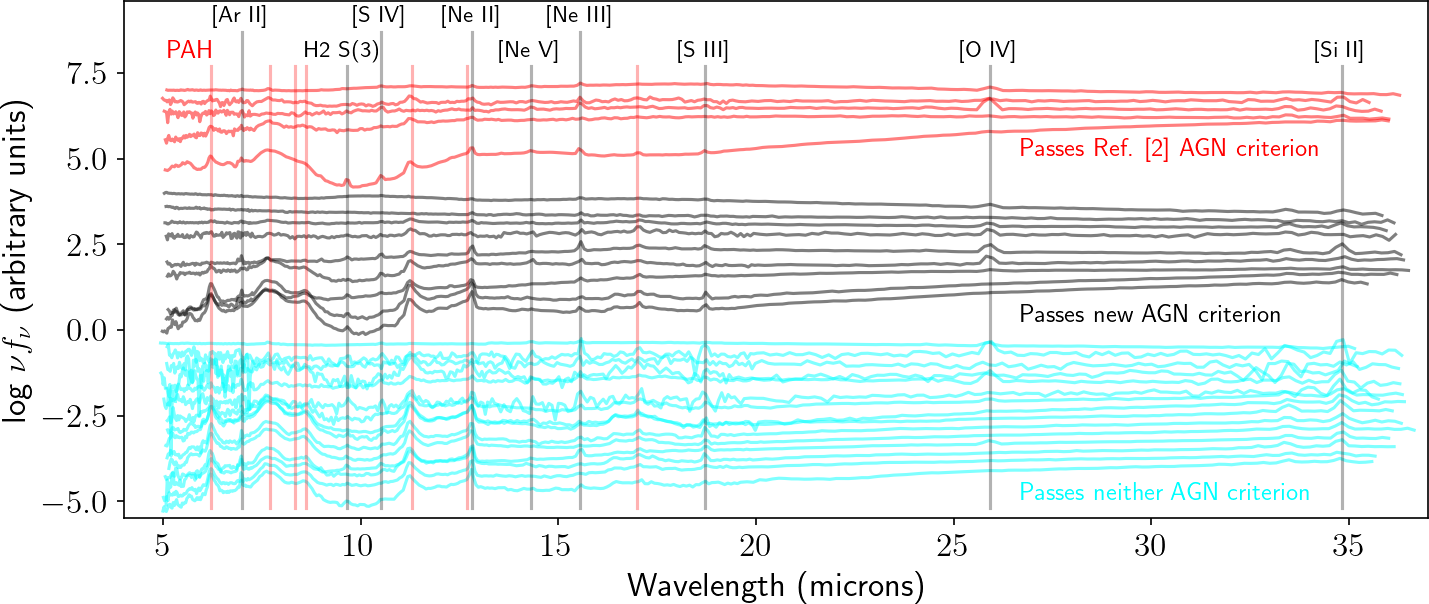
\includegraphics[width=0.92\textwidth]{all-spitzer.png}
    \caption{
\label{fig:spitzer} \small Spitzer spectra for MaNGA galaxies
from \cite{lambrides}. They are colored by W1$-$W2 (increasing
in color from blue to red), and they are offset by arbitrary
amounts for clarity. For various spectra, one can see 
the silicon absorption  feature, PAH features, [O IV] 26 $\mu$m, 
and some high ionization lines such as [Ne V].
}
\end{figure}

The spectra provide mid-IR indicators that can be used to test our new
criterion.  The PAH 6.2 $\mu$m equivalent and the silicon absorption
depth have been measured for these spectra by \cite{lambrides}.  The
PAH measurement is strong if the galaxy is dominated by star
formation, but weak if the emission is dominated by the AGN
\cite{sajina22a}.  The silicon absorption is typically a signature of
an AGN.  We will also measure other signatures where possible, which
include [O IV] 26 $\mu$m, [Ne V] 14.3 $\mu$m, [S IV] 10.5 $\mu$m, and
other emission line fluxes.  We will examine the relationship between
W1$-$W2, these signatures, and (for the 30 galaxies for which they are
available) the MaNGA based estimates of stellar metallicity, star
formation rate, and stellar mass. From these relationships we will
attempt to determine the reliability of W1$-$W2 as an indicator of the
presence of an AGN, paying particular attention to whether candidate
AGN introduced by our new criterion are convincingly mid-IR AGN based
on these indicators.

The Spitzer spectra will also allow us to assess and refine our SED
fitting to the WISE data. We will expand the SED analysis to include
the NSA galaxies in the sample of \cite{lambrides}.  Then for both the
NSA subsample and the MaNGA galaxies we will directly compare the
spectra we fit to WISE to the detailed Spitzer spectra, to determine
whether the balance of PAH and hot dust emission is accurate. We will
use these results to refine our choice of dust emission templates in
our SED fitting. For the subset of spectra that are in MaNGA we can
also determine the extent that physical properties such as stellar
mass and star formation rate affect the SED modeling and can be used
to improve its agreement with the Spitzer data.

\subsection{Fitting Eddington Ratio Distributions}
\label{sec:erd}

{\bf The work described above will position us to achieve the main
  goals of the proposal: to measure mid-IR luminosity and Eddington
  ratio distributions as a function of galaxy properties, in
  particular stellar mass ($M_\ast$), velocity dispersion ($\sigma$),
  and specific star formation rate (sSFR).}

We will calculate the mid-IR luminosity distributions using a standard
maximum likelihood technique utilizing the mid-IR luminosities and
upper limits observed for the sample. Specifically, we seek the
quantity:
\begin{equation}
\Phi\left(L_{\rm IR} | X\right)
\end{equation}
where $X$ is $M_\ast$, $\sigma$, or sSFR. The advantage of the MaNGA
sample is that these quantities are known extremely reliably in ways
that are insensitive to the presence or absence of the AGN. We will
use at least two choices of parametrization---a broken power law and a
Schechter function, each of which can be characterized by a set of
parameters $\vec{\theta}$.

Within any given model, we will maximize the log-likelihood, which can
be expressed as:
\begin{equation}
\ln \mathcal{L} = \sum_i \ln p_i\left(L_{{\rm IR},\,i}  | X\right),
\end{equation}
where for detected AGN:
\begin{equation}
p_i = \Phi\left(L_{{\rm IR}, i}; \vec{\theta} \right)
\end{equation}
and for non-detected AGN:
\begin{equation}
p_i = \int_0^{L_{{\rm IR, lim},\,i}} {\rm d}L \Phi\left(L; \vec{\theta}\right),
\end{equation}
where $\Phi(L)$ is a model for the luminosity function with
parameters $\vec{\theta}$, and $L_{{\rm IR, lim},\,i}$ is the upper limit 
on the AGN mid-IR luminosity for each galaxy $i$.
The upper limits are critical for this study since they allow
us to utilize the many non-detections, which can provide important
constraints on the distribution.

Given ur sample size, we expect not to be able to determine the full
joint dependence on multiple properties (i.e. on all three of
$M_\ast$, $\sigma$, and sSFR together). Instead, based on the results
of fitting each dependence separately, we will search for residual
dependence on the other two properties. In this way we will examine
whether one dependence is primary and the others merely secondary to
it, or whether the dependence is more complicated.

To calculate Eddington ratios we need to infer both the bolometric
luminosity and the black hole mass (which sets the limiting Eddington
luminosity). In our context, the absolute level of the Eddington ratio
is less important than that we provide some appropriate scaling of the
AGN emission as a function of black hole mass.  For the bolometric
luminosity we will use the nonlinear relation of \cite{stern15a}
between mid-IR 6 $\mu$m luminosity and X-ray luminosity, and assume a
factor of 20 between X-ray luminosity and bolometric
luminosity. Although this approach is susceptible to variations in the
bolometric-to-mid-IR luminosity ratio, we note that the sample we
develop will be well matched to future public eROSITA catalogs, in
order to help better calibrate this relationship.

We will infer the black hole mass using the central velocity
dispersion from the MaNGA data and the $M_{\rm BH}$--$\sigma$
relation, which is measured at high precision.  A major advantage of
our sample relative to others (particularly larger but lower
signal-to-noise ratio samples like SDSS Legacy and the upcoming DESI
Bright Galaxy Survey) is the excellent measurements of $\sigma$ of the
host galaxy. We will use several alternative versions of the $M_{\rm
  BH}$--$\sigma$ relation, including versions with second parameter
dependencies (e.g. \cite{kormendy13a, vandenbosch16a, shankar16a}).

We then can define the Eddington ratio in the usual way as $\lambda =
L_{\rm bol} / L_{\rm Edd}$, where $L_{\rm Edd}\propto M_{\rm BH}$.
With the Eddington ratios $\lambda$ and upper limits on Eddington
ratios in hand, we will use the same techiques as for the luminosity
distribution to infer the Eddington ratio distribution and its
dependence on galaxy properties. We will explore the effects of
systematic differences methodology for the bolometric luminosity and
black hole mass determination on the overall results.

Based on the work of \cite{dasyra08a}, we also plan to use the Spitzer
spectra to validate these estimates.  The velocity dispersion of the
high ionization lines can yield independent indicators of the black
hole mass, which we can compare to the velocity-dispersion based
estimates. Estimates of the 15 $\mu$m AGN continuum from these spectra
and the high ionization line measurements will also produce estimates
of the bolometric luminosity \cite{dasyra08a, shen20a}, which we will
compare to the WISE-based estimators.

%\subsection{Comparison with Narrow Line AGN Manifestations}
%\label{sec:other}
%
%AGN manifest in a number of different ways. The work proposed here is
%part of a larger effort to study local AGN in optical narrow lines,
%mid-IR, X-rays, and the radio, accounting for the different selection 
%effects in each one. {\bf To support our understanding of the 
%mid-IR luminosities will characterize the
%relationship between the mid-IR luminosities and optical narrow line 
%[O III] luminosities accounting for upper limits in each case}.

%Previous efforts in this area have shown that searching for AGN in
%different manifestations yield overlapping but different samples of
%AGN \cite{hviding22a}. Figure \ref{fig:bpt} investigates the
%signatures of optical narrow line emission for these candidates; in
%summary, although the mid-IR AGN preferentially present as narrow line
%Seyferts, about half do not, and vice-versa. There are some intriguing
%patterns in the diagram, such as a population of objects that appear
%to be low metallicity star forming galaxies according to emission
%lines, but have high enough W1$-$W2 to pass any AGN selection
%criterion (the cyan points near the left of the diagram).
%
%But we cannot interpret this diagram without understanding the upper
%limits AGN-related [O III] luminosity {\it and} the mid-IR upper
%limits determined from this work. For the former, in previous work we
%have implemented a method based on the work of \cite{trump15a} to
%determine the [O III] upper limits \cite{liu21a}, which we will use
%here. By taking to account these upper limits, we can determine
%whether mismatch between mid-IR AGN candidates and optical narrow line
%Seyfert galaxies is merely due to selection effects or reflects a true
%heterogeneity in AGN manifestations.
%
%Studies of this relationship in the past rely on using very luminous
%AGN which outshine their galaxies (e.g. \cite{lamassa12a}). Studies of
%lower luminosity mid-IR AGN and [O III] have not explored this
%relationship because they did not remove host galaxy contamination to
%the mid-IR or determine the selection effects in either quantity
%(e.g. \cite{hviding22a}). We will advance this area with a more
%complete analysis that addresses this question.

\subsection{K-correction and SED fitting software}

This work relies on and contributes to a publicly available utility
for fitting SEDs called {\tt kcorrect} \cite{blanton07b}, recently
released in Python.  We will contribute to the development of {\tt
  kcorrect} to include AGN emission templates in the mid- and far-IR.
This will aid in the identification of AGN in UV, optical, and IR data
and in the determination of their luminosities, and make the tools we
use for this work publicly available.

%\begin{figure}[h!]
%\begin{center}
%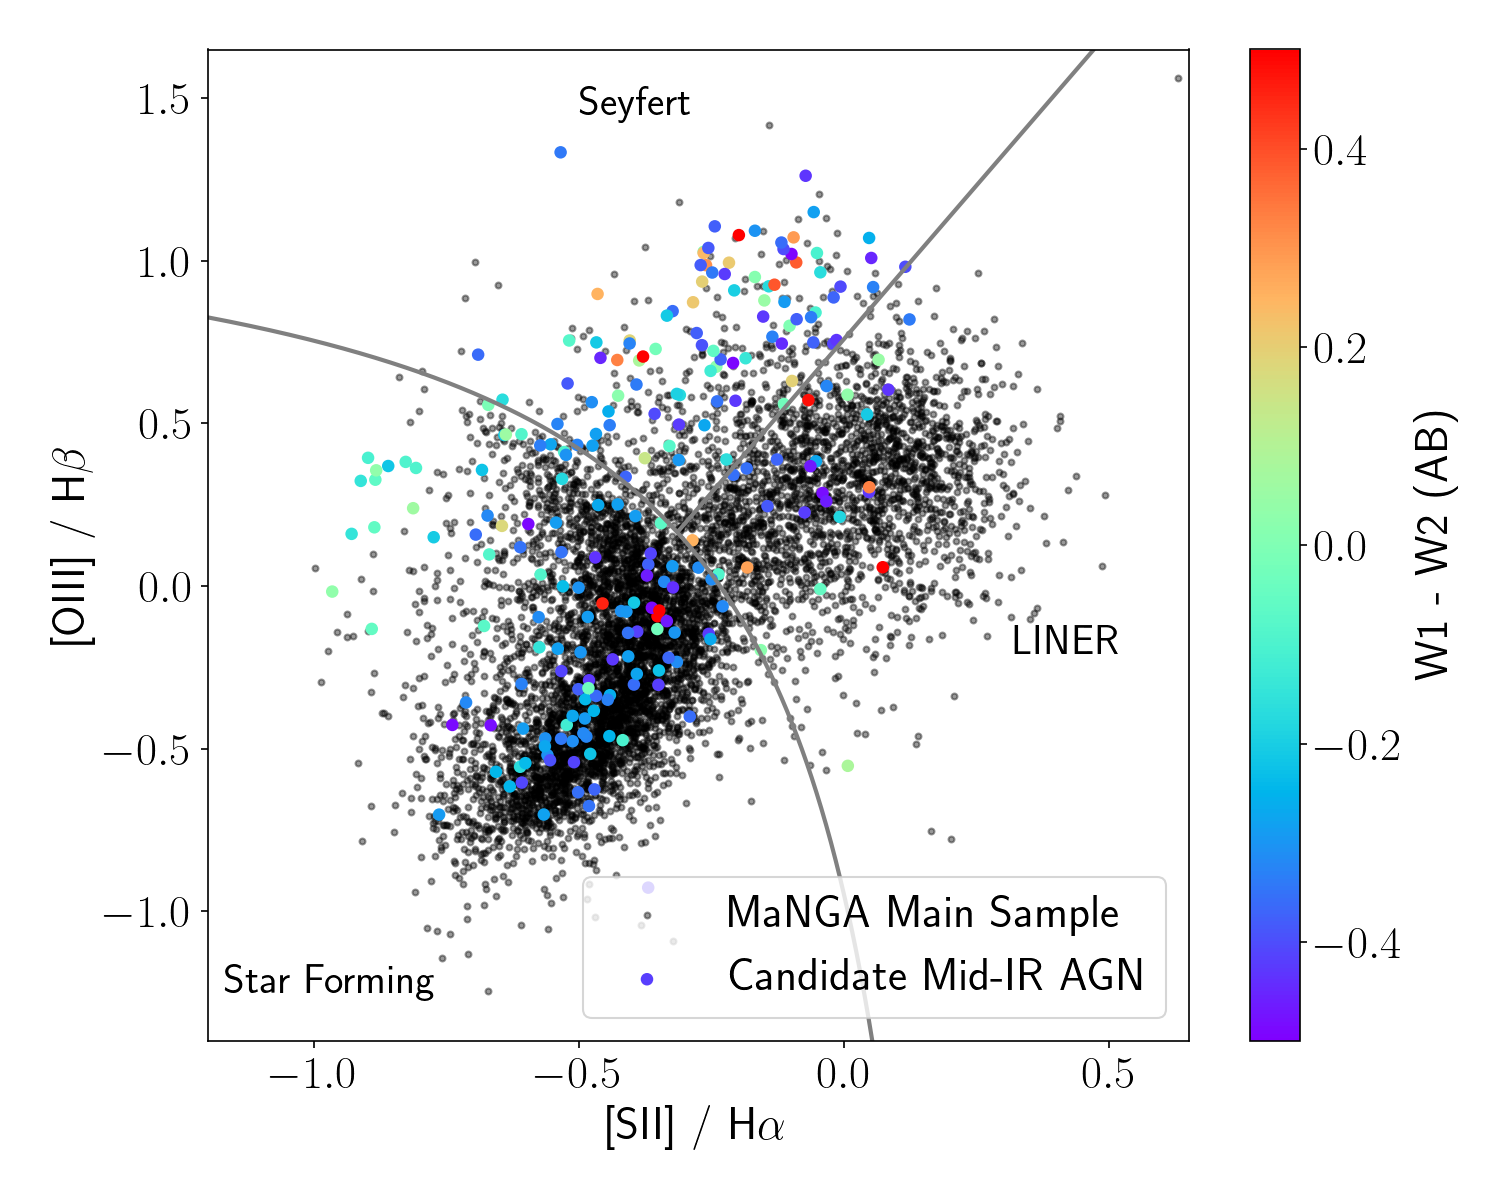
\includegraphics[width=0.91\textwidth]{bpt-agn.png}
%\end{center}
%\caption{\label{fig:bpt} The [S II]-based line ratio diagram
  %\cite{veilleux87a} with standard divisions into ionization source
  %classes: star formation, LINER, and Seyfert \cite{kewley06a}.  We
  %expect that essentially all AGN with substantial hot dust emission
  %will also have an ionized narow line region, whose emission line
  %ratios would be in the Seyfert region of this diagram if there was
  %not competing emission from other components of the galaxy. The
  %mid-IR candidates are shown colored according to W1$-$W2; note that
  %there is no strong tendency for redder colors to be in the Seyfert
  %region of the diagram. Of the mid-IR candidates, only about half
  %have Seyfert classifications; the same is true for the more
  %conservative mid-IR criterion of \cite{assef18a}. In this work we
  %will use upper limits we have previously determined on narrow line
  %emission to determine the reason for the mismatch in this diagram.}
%\end{figure}

\section{Objections, Uncertainties, Difficulties, and Their Mitigation}
\label{sec:difficulties}

\fbox{\parbox{\textwidth}{\bf The goals of this proposal are ambitious
    and carry some risk regarding whether we can identify as many
    mid-IR AGN as we hope and measure their luminosities well.  In
    this section we describe how we will mitigate these risks and
    assess the performance of our methods. Additionally we argue that
    even if we cannot increase the local mid-IR AGN population as
    dramatically as planned, that would imply the discovery of
    interesting new populations of galaxies that we would study.}}

\noindent{\bf Why look in the mid-IR?} The mid-IR provides a unique
view of the population of AGN, in particular relative to the X-rays
and optical detection. It reveals obscured AGN whose emission is not
evident in other bandpasses \cite{sajina22a}. In addition, the
mid-IR-emitting AGN present promising targets for follow-up
observations, since mid-IR spectroscopy and time variability can yield
important diagnostics of the gas and dust structures deep inside the
galactic nuclei \cite{goold23a}. However, we do not argue that the
mid-IR should be favored over other wavelength ranges; rather, the
point is that there is so much variation among AGN manifestations that
no single window onto their activity is sufficient. We seek to
understand the mid-IR {\it as part of} a broader attack on local AGN
demographics.

\noindent{\bf Are the AGN candidates actually AGN?} Our criterion for
selecting AGN from W1$-$W2 includes much bluer colors than even the
most inclusive color cuts used by others (e.g. from \cite{assef18a}).
We need to consider whether there are non-AGN SEDs that can explain
W1$-$W2 colors that are offset to the red relative to most galaxies.
Low metallicity star burst components of the host galaxy can redden
the W1$-$W2 color across our threshold; for example,
\cite{hainline16a} argue that the W1$-$W2 color for starburst dwarf
galaxies can exceed even the more conservative criteria of
\cite{stern12a}.  Alternatively, in galaxies with intermediate age
stellar populations but little recent star formation, hot dust
envelopes of asymptotic giant branch stars can contribute to the W2
band and again lead to redder W1$-$W2 \cite{villaume15a}. For our
sample, with stellar masses mostly $> 10^9$ $M_\odot$ and redshifts
$z<0.15$, our {\it a priori} expectation is that these effects are
unlikely but possible---for example, the cyan points discussed in
Figure \ref{fig:bpt} are possibly low metallicity star bursts. We can
use the detailed MaNGA spectra to characterize metallicities and star
formation histories, as well as the Spitzer spectra where available,
which can help diagnose these unusual cases. If we can validate that
our new criterion reliably identifies AGN, we will have increased the
sample of mid-IR AGN by a large factor. Alternatively, if some of the
mid-IR AGN candidates can be shown to be non-AGN galaxies with unusual
star formation histories, that discovery will also be worth pursuing.

\noindent{\bf Can we measure AGN luminosities accurately?} To measure
the mid-IR AGN luminosities it is necessary to account for host galaxy
luminosity, even for the more extreme W1$-$W2 colors
\cite{lacy15a}. This task is more demanding for our expanded sample
with small color offsets from the host galaxy distribution. Our SED
fitting method described in Section \ref{sec:measurements} has
intrinsic uncertainties that we will have to assess. As we described,
we will determine statistical uncertainties using a Monte Carlo
method.  In addition, we will explore a variety of stellar population
model assumptions, star formation related PAH emission assumptions,
and AGN SED model assumptions, and test the effects of systematic
calibration offsets in the photometry, to determine the level of
systematic errors that the inferred luminosities suffer from. As
described in Section \ref{sec:spitzer}, we will use the Spitzer
spectra to assess and refine the SED fits. A further reality check
will be to compare the luminosities to the [O III] luminosity from
MaNGA; we expect at least for the more luminous cases that these
luminosities will be correlated with each other.

\noindent{\bf Is our model for selection effects sufficiently good?}
For the inference of luminosity and Eddington ratio distributions, we
need to accurately understand the selection effects on detecting
AGN. But if the mid-IR emission SED changes systematically with
Eddington ratio or galaxy host properties in the range we are
studying, our model of selection effects needs to account for
this. For example, the dust temperature distribution (which is
plausibly related to Eddington ratio and gas metallicity) changes the
mid-IR emission spectrum. As described in Section
\ref{sec:measurements}, we will determine the typical AGN SED fits as
a function of sSFR, stellar mass, and inferred Eddington ratio in
order to test for this variation, and its effects on our inferred
distributions.  We will also use the Spitzer spectra to explore this
variation.

\section{Project Plan and Timeline\label{sec:plan}}

The bulk of this work will be performed by a Graduate Research
Assistant (GRA) as their PhD thesis.  The PI will mentor the GRA and 
assist in data analysis, writing, and interpretation. An undergraduate
researcher will also assist in data analysis and data vetting.

\begin{ditemize}
\item {\it Year 1}: 
\begin{ditemize}
\item Develop AGN and galaxy SED fitting to determining AGN
  luminosities and upper limits from the WISE data.
\item Use Spitzer spectra to refine classification criteria, and to
  tune SED templates for accurately determining of 6 $\mu$m AGN
  luminosities and upper limits.
\item Publish catalog of AGN luminosities and upper limits, and
  methodology paper on fitting AGN and galaxy SEDs.
\end{ditemize}
\item {\it Year 2}: 
\begin{ditemize}
\item Fit Eddington ratio distribution models using mid-IR AGN
  luminosities and upper limits.
\item Publish inferred Eddington ratio distributions as a function of
  host galaxy stellar mass and SFR.
\item Publish comparison of mid-IR luminosities to [O III] narrow-line
  luminosities, to constrain the joint distribution of these emission
  properties. 
\end{ditemize}
\end{ditemize}

\section{Open Science and Data Management Plan\label{sec:data}}
\vspace{-6pt}

The data products will be WISE band luminosities and uncertainties,
AGN classifications, AGN mid-IR luminosities, uncertainties, and upper
limits, and SED fitting results for all 10,000 MaNGA galaxies.  We
will also produce SED fitting to the Spitzer spectra used. These data
will be stored as FITS files and distributed publicly.  We will submit
them to SDSS to publish as a Value Added Catalog in a future data
release.

The software pipelines specific to this project, including
contributions to {\tt kcorrect}, will be version controlled using {\tt
  git} and distributed in a GitHub repository. They will be licensed
under the 3-clause Berkeley Software Distribution (BSD-3) license.

\clearpage
\section{References}\label{sec:refs}

\printbibliography[title=~]

\clearpage
\section{Budget Narrative}\label{sec:budget}

\noindent {\bf Senior Personnel:} The PI is requesting 1.0 month of
summer salary for each of the 2 years of the project.  The PI is
responsible for the overall management of the project. The PI will
supervise the GRA and undergraduate and will assist in the writing,
data analysis, and interpretation.

\noindent {\bf Other Personnel:} Graduate Research Assistant (GRA):
Funds are requested for 2 academic years (AY) plus 2 summers. The GRA
will develop the software and perform the analysis described in the
proposal. Undergraduate Research Assistant (UGRA): Funds are requested
for an hourly research position. The UGRA will work with the GRA and
assist in the data analysis and data vetting.

\noindent {\bf Fringe Benefits Rate:} A fringe benefits rate 
applies to the PI salary and the undergraduate student salary. % 31%

\noindent {\bf Capital Equipment:} Funds are requested in Year 1 for 
dedicated computer  servers with which to perform the analysis (\$5,000 each
for two Dell PowerEdge R7525 Servers, with 2 16-core processers with 128M 
of cache, 4 Tb of local disk,  and 64 Gb of memory).

\noindent {\bf Domestic Travel:} Funds are requested for attendance at
one domestic conference for the GRA in each year. We assume \$1500 for
a 4-day conference (\$200 for registration fee, \$500 for airfare,
\$150/night for lodging, and \$50/night per diem).

\noindent {\bf Foreign Travel:} Funds are requested for attendance at
one foreign conference for the GRA in each year. For each conference
we assume \$1500 for a 4-day conference (\$200 for registration fee,
\$500 for airfare, \$150/night for lodging, and \$50/night per diem).

\noindent {\bf Publications:} We anticipate two 10-page journal
articles each year. Based on prior experience with the AAS Journals,
the typical publication cost will be \$1500 per paper in 2023 dollars.

\noindent {\bf Other Direct Costs:}
Graduate students receive tuition remission. % charged at 37% of
                                % graduate student salary in lieu of
                                % fringe benefits

\noindent {\bf Rates:} Senior personnel salaries increase XX\%
annually, while OTPS costs increase YY\% per year. % XX = 4, YY = 2.5

\noindent {\bf Indirect Costs:} An indirect cost rate has been
negotiated with DHHS, agreement dated October 6, 2021.
%The agreed upon
%rate for Facilities and Administration costs (F\&A) is 61\% as of FY
%2024 and thereafter.
The MTDC base excludes capital equipment, tuition
remission, participant support costs, and subcontracts beyond the
first \$25,000. 

\clearpage
\section{Summary of Work Effort}\label{sec:effort}

%The work will be divided as described in the table below.

\begin{table}[h!]
\centering
\caption{Personnel and Work Effort (all project years)\label{table:effort}} 
%\caption{Table of Work Effort\label{table:effort}} 
\begin{tabular}{lccc}
\\
\hline
& {\bf Funded Effort} & {\bf Unfunded Effort} & {\bf Total Effort} \\
{\bf Role} & {\bf (months / year)} & {\bf (months / year)} 
& {\bf (months / year)} \\
\hline
\hline
PI & 1 & 0 & 1 \\
Graduate Student & 12 & 0 & 12 \\
Undergraduate Student & 2 & 0 & 2 \\
\hline
\end{tabular}
\end{table}

\clearpage
\section{Budget Details}
\label{sec:budget-details}

\noindent {\bf Senior Personnel:}\\
{\it excluded as requested}

\noindent {\bf \it Other Personnel:}\\
\noindent {\bf Graduate Research Assistant (GRA):}\\
{\it excluded as requested}

\noindent {\bf Fringe Benefits Rate:}\\
{\it excluded as requested}

\noindent {\bf Capital Equipment:}\\
Year 1: \$10,000\\
Year 2: \$0

\noindent {\bf Domestic Travel:}\\
Year 1: \$1,500\\
Year 2: \$1,538

\noindent {\bf Foreign Travel:}\\
Year 1: \$1,500\\
Year 2: \$1,538

\noindent {\bf Publications:}\\
Year 1: \$3,000\\
Year 2: \$3,075

\noindent {\bf Other Direct Costs (Tuition Remission):}\\
Year 1: \$16,238\\
Year 2: \$16,806

\noindent {\bf Indirect Costs:}\\
{\it excluded as requested}

\end{document}
